% Preamble
% ---
\documentclass{article}

% Packages
% ---
\usepackage{amsmath} % Advanced math typesetting
\usepackage[utf8]{inputenc} % Unicode support (Umlauts etc.)
\usepackage[english]{babel} % Change hyphenation rules
\usepackage{hyperref} % Add a link to your document
\usepackage{graphicx} % Add pictures to your document
\usepackage{listings} % Source code formatting and highlighting
\usepackage{amssymb} % Extra math symbols
% ---
\graphicspath{{./images/}}
%

\title{Mixed-precision Block QR Decomposition on GPU}
\author{Jaidon Lybbert}
\date{\today{}}

\begin{document}

\maketitle{}
\tableofcontents{}

\section{QR Decomposition}
\paragraph{}
The QR decomposition of an m-by-n matrix $A$ with $m>n$, is the matrix product $A = QR$, where $Q$ is an 
m-by-n unitary matrix, and $R$ is upper triangular.

\subsection{Matrix Q}
\paragraph{}
The matrix $Q$ is a transformation which preserves inner products of column vectors of $R$. If the 
inner product space is real, the matrix $Q$ is equivalently orthogonal. One possibility of such a 
transformation is a rotation.
\paragraph{}
Another possibility of such an orthogonal transformation is a reflection. The matrix $Q$ in general 
is a combination of rotations and reflections.

\subsection{Matrix R}
\paragraph{}
The matrix $R$ is upper triangular, a form which has the following useful properties: (I) the determinant is equal to the product of the diagonal elements, (II) the eigenvalues are equal to the diagonal elements, (III) given the linear system $Rx = b$ it is easy to solve for $x$ by back substitution.

\section{Computation}
\paragraph{}
In order to compute the decomposition of $A$, the matrix is iteratively transformed by unitary matrices $\{U_i : 0 < i < k\}$ until the product is upper triangular. This upper triangular matrix is the matrix $R$ in $A = QR$
\begin{equation}
R = U_kU_{k-i} \dots U_1A.
\end{equation}
\paragraph{}
It follows, that the matrix $Q$ is composed of the set of inverse transformations
\begin{equation}
Q = U_{1}^{T}U_{2}^{T} \dots U_{k}^{T}.
\end{equation}
\paragraph{}
The key to solving for $R$ is to choose transformations $U_i$ which produce zeros below the diagonal of the matrix product
\begin{equation}
P = U_{i} \dots U_1A,
\end{equation}
and can iteratively be applied to converge to $R$ as quickly as possible. Two choices for $U_i$ are Householder reflections, and Givens rotations.

\subsection{Householder Reflections}
\paragraph{}
The Householder reflection is a unitary transformation represented by a matrix $H\in\mathbb{R}^{N\times{}N}$ which reflects a vector $x\in\mathbb{R}^N$ across a hyperplane defined by its unit normal vector $\{w\in\mathbb{R}^N: \|w\|=1\}$. The transformation matrix is given by
\begin{equation}
H = I - 2\mathbf{ww}^T
\end{equation}
where $I\in\mathbb{R}^{N\times{}N}$ is the identity matrix. \cite{bhaskar86}

\begin{figure}[h]
\centering
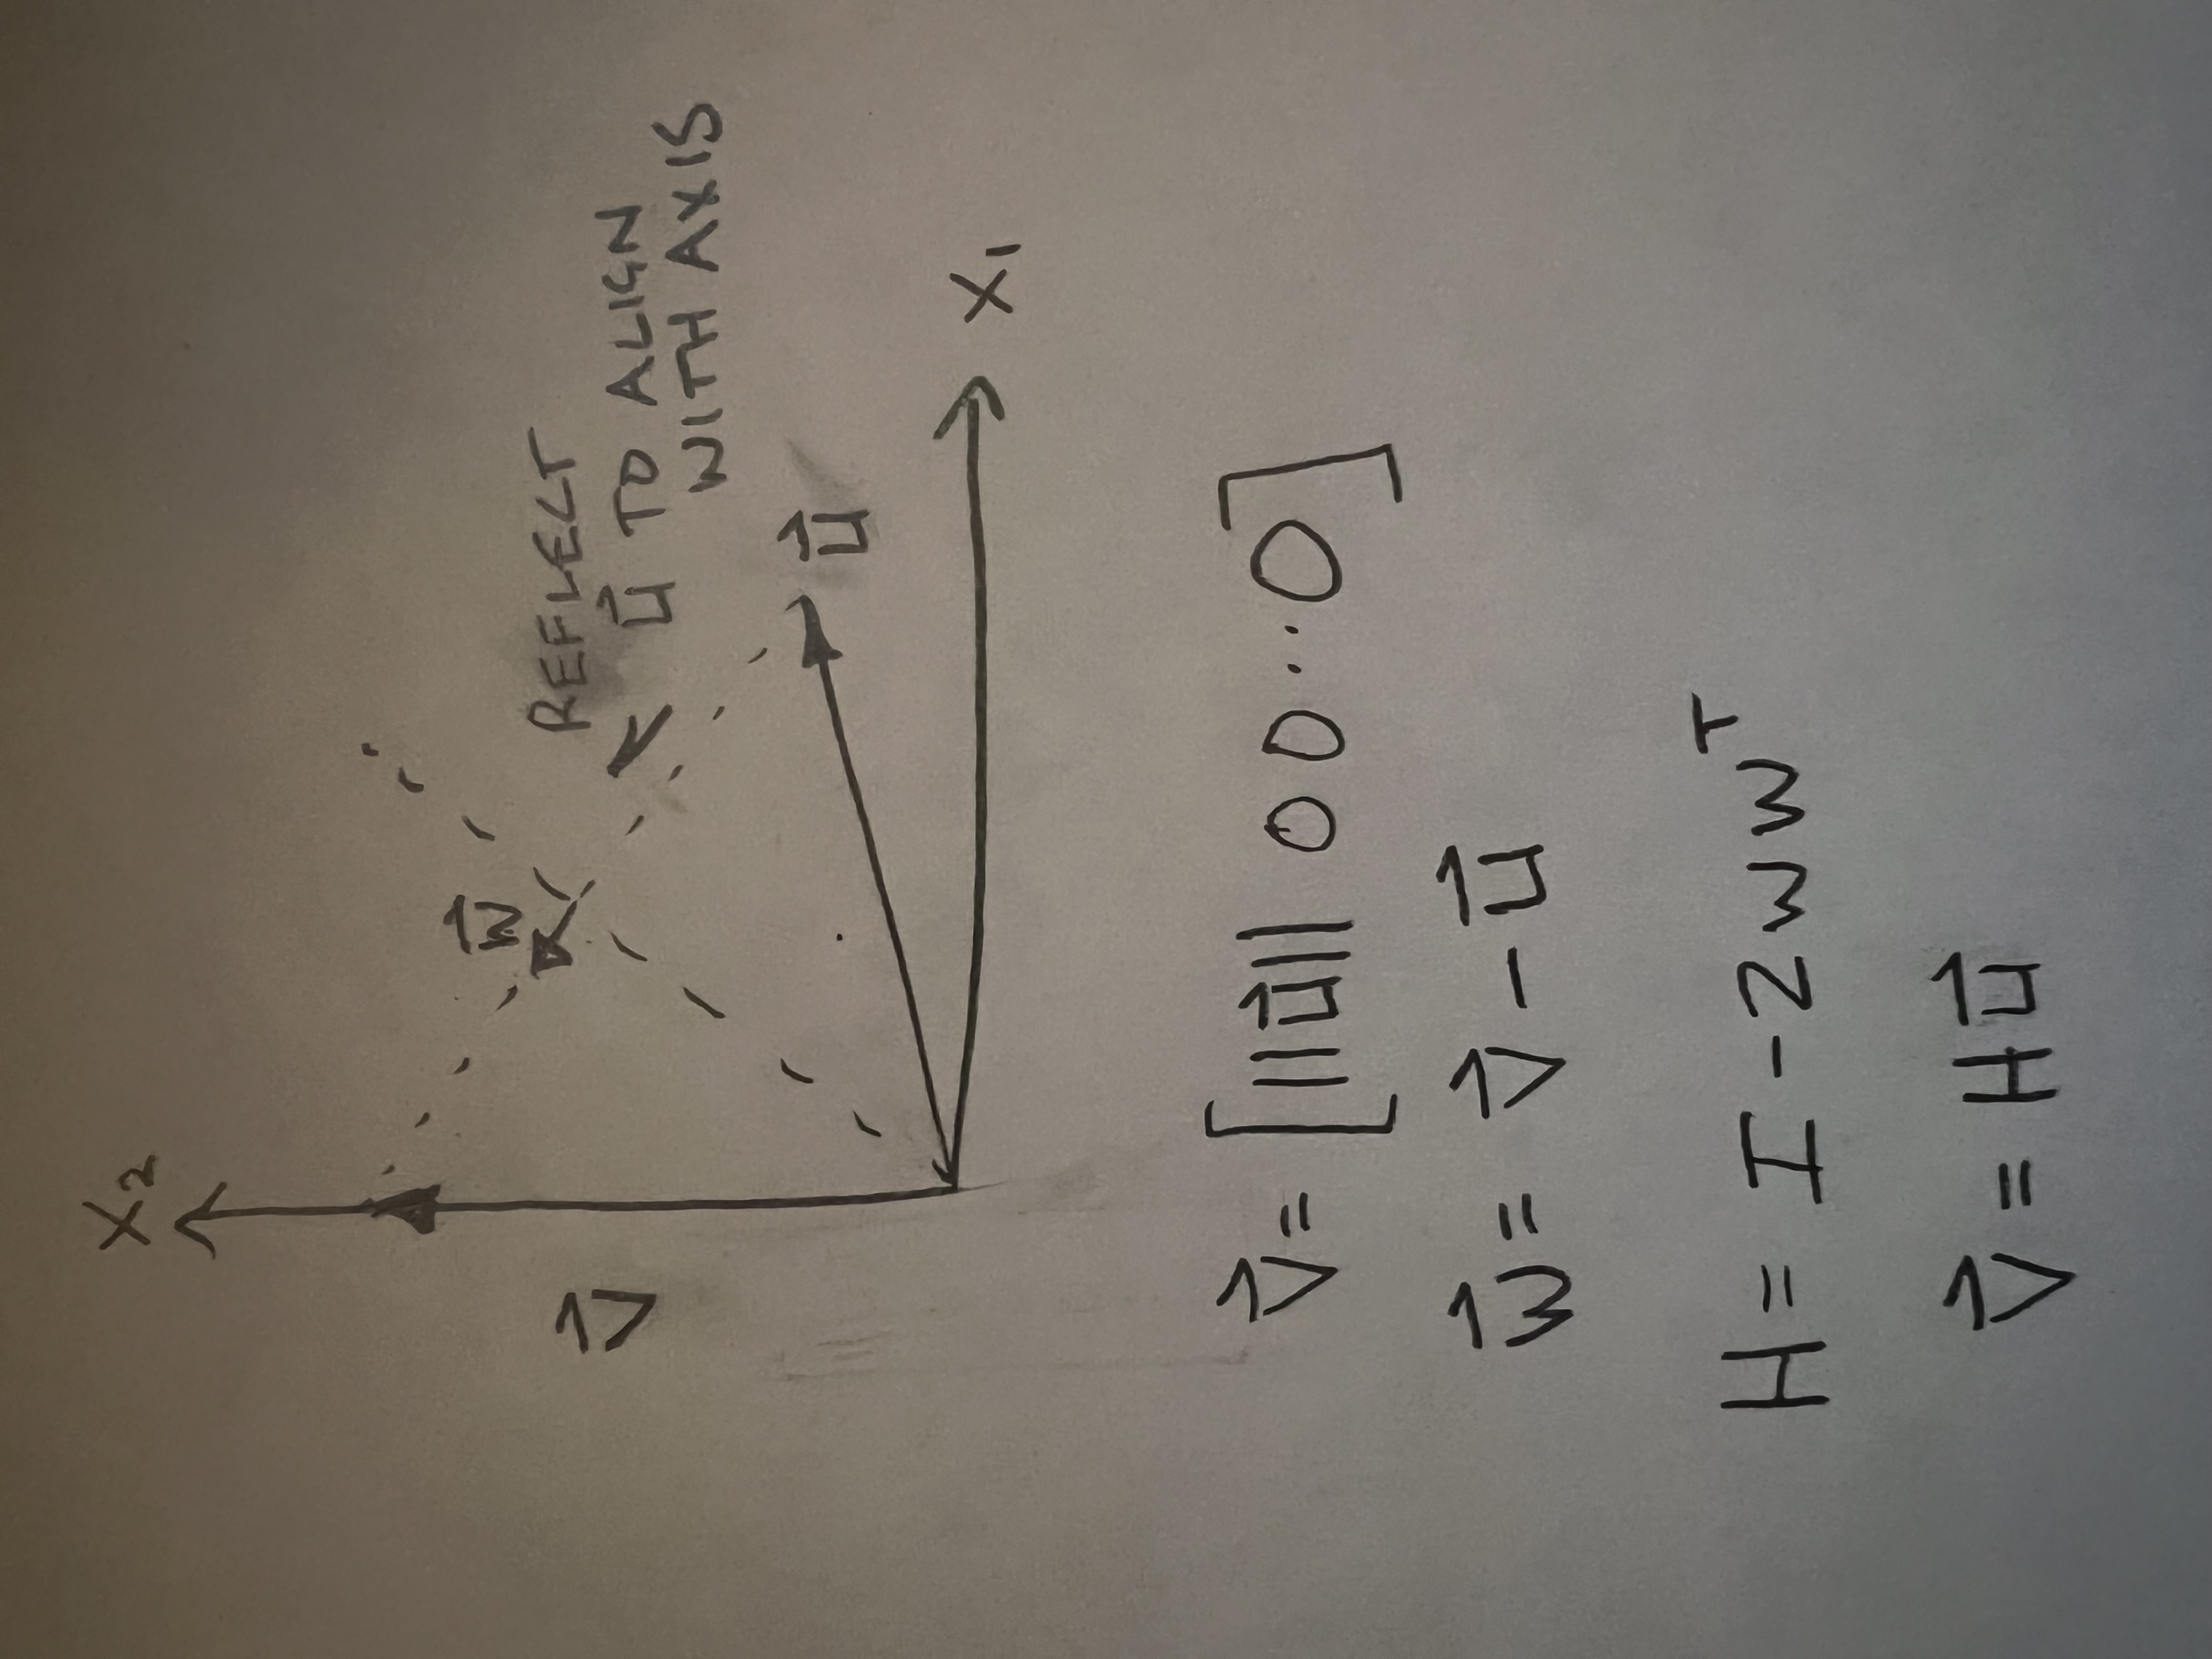
\includegraphics[width=75mm, angle=-90]{Householder2}
\caption{Geometric illustration of the reflection of a vector to an axis. The result of this transformation is that the vector now only has one non-zero component.}
\end{figure}

\paragraph{}
In order to get the upper triangular matrix $R \in\mathbb{R}^{N\times{}N}$ given a matrix $A \in\mathbb{R}^{M\times{}N}$ using householder reflections, each column is treated in sequence left to right. 
\pagebreak
\begin{figure}[h]
\centering
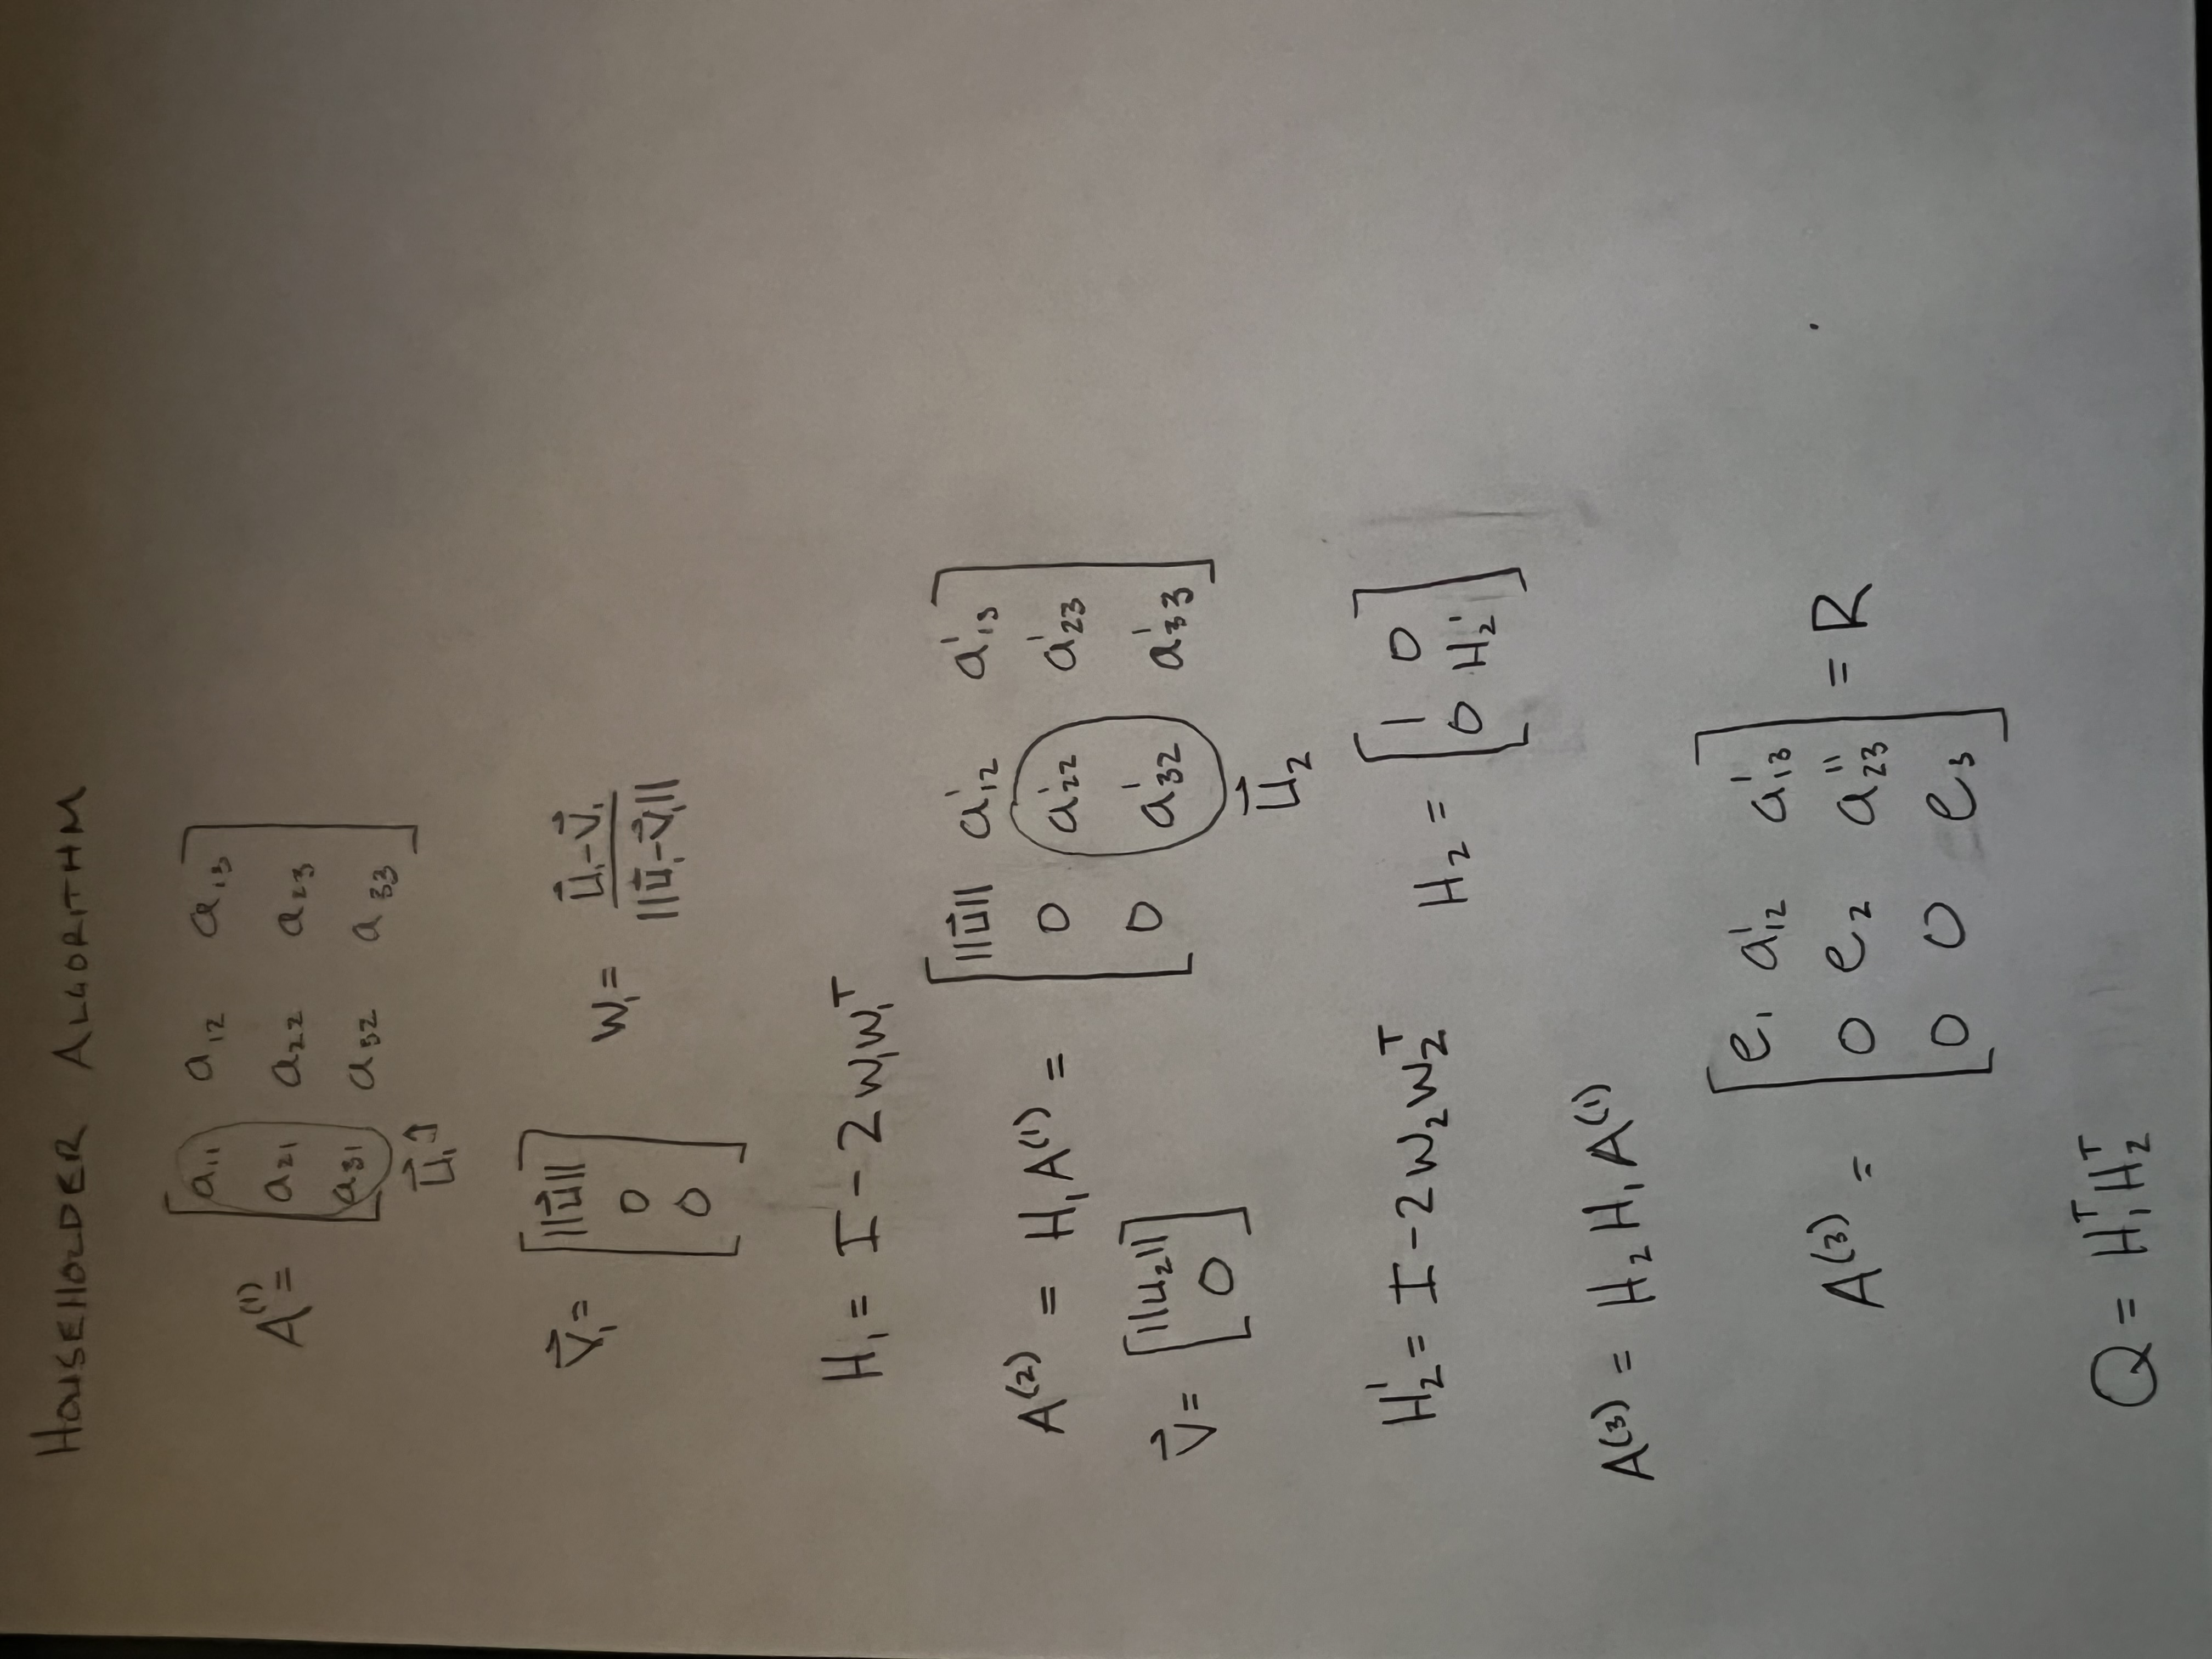
\includegraphics[width=140mm, angle=-90]{Householder3}
\caption{QR factorization algorithm with Householder reflections}
\end{figure}

\subsection{Givens Rotations}
\paragraph{}
A Givens rotation is a unitary transformation which rotates a vector $x$ counter-clockwise in a chosen plane. For example, possible Givens rotation matrices in $\mathbb{R}^4$ include
\begin{equation}
\begin{bmatrix}
1 & 0 & 0 & 0\\
0 & c & -s & 0\\
0 & s & c & 0\\
0 & 0 & 0 & 1
\end{bmatrix},
\begin{bmatrix}
c & -s & 0 & 0\\
s & c & 0 & 0\\
0 & 0 & 1 & 0\\
0 & 0 & 0 & 1
\end{bmatrix}, or
\begin{bmatrix}
1 & 0 & 0 & 0\\
0 & 1 & 0 & 0\\
0 & 0 & c & -s\\
0 & 0 & s & c
\end{bmatrix},
\end{equation}
where $c = \cos{\theta}$ and $s = \sin{\theta}$. Each of these examples have the effect of rotating the vector in different planes.
\paragraph{}
The Givens rotation is parallelizable because it effects only two dimensions of the input vector. For example, the second and last transformations above could 
simultaneously be computed on the vector $x$, then the results combined by selecting the first 2 
dimensions of the first result, and the second two dimensions of the second result.

\paragraph{}
A Givens rotation can easily be computed to introduce zeros in the matrix $P$. The scalars $c$ and $s$ 
can be computed directly from elements in $P$ in order to zero out targeted elements. For 
example, say we want to zero out element $a_{21}$ in the matrix
\begin{equation}
P = 
\begin{bmatrix}
a_{11} & a_{12} & a_{13}\\
a_{21} & a_{22} & a_{23}\\
a_{31} & a_{32} & a_{33}
\end{bmatrix}.
\end{equation}
\paragraph{}
We target the second dimension of the column vector, so we rotate on the plane spanned by 
the first two dimensions. We don’t choose the plane spanned by the second and third dimensions, 
because we would end up losing the zero in the third row in the process. The Givens rotation to rotate 
on this plane is of the form
\begin{equation}
G = 
\begin{bmatrix}
c & -s & 0\\
s & c & 0\\
0 & 0 & 1
\end{bmatrix}
\end{equation}
which will leave the third row of $P$ unmodified. We are aligning the column vector with the axis of the first 
dimension, making the component of the vector along the second dimension zero. Below is a geometric 
illustration of the rotation.

\begin{figure}[h]
\centering
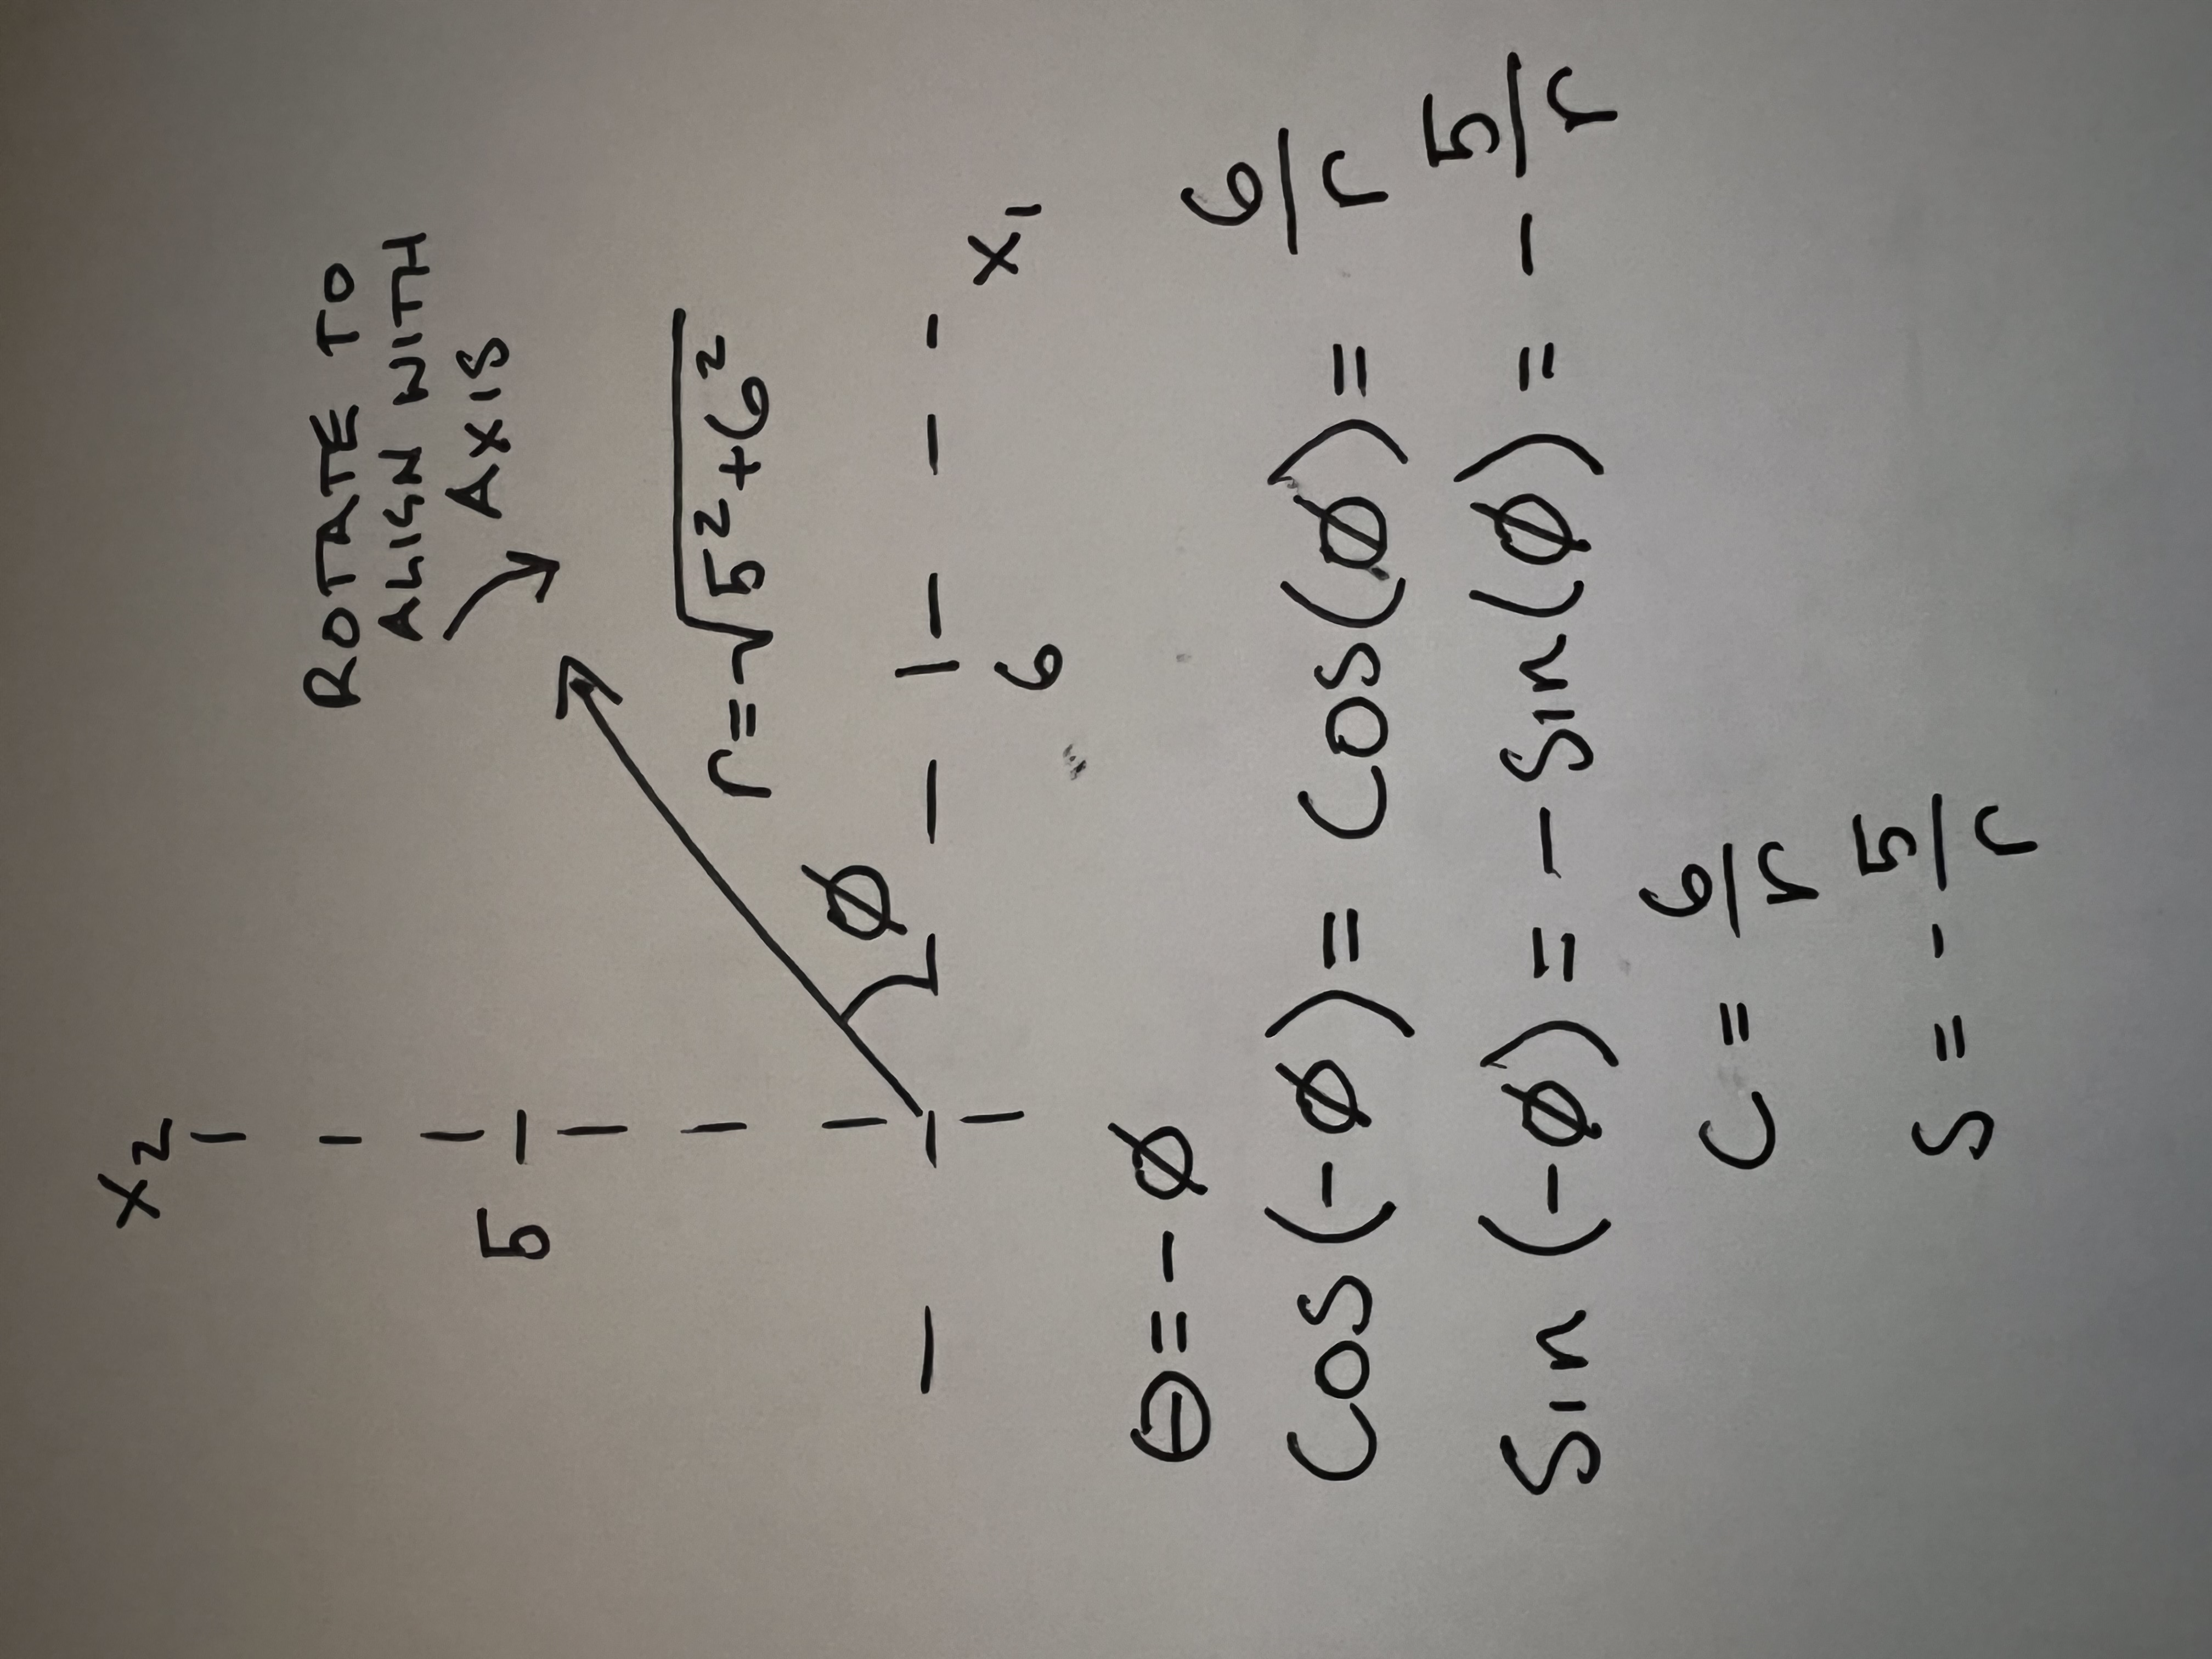
\includegraphics[width=75mm, angle=-90]{Givens1}
\caption{Geometric illustration of the rotation of a vector in $\mathbb{R}^3$ about the axis of basis vector ${x3}$ to align with the basis vector ${x1}$. The result of this transformation is that the component of the transformed vector in the direction of the basis vector $x2$ is zero, corresponding to a zero introduced in the transformed matrix.}
\end{figure}

\paragraph{}
The scalars $c$ and $s$ of matrix $G$ are computed directly from the values in matrix P by the equations 
\begin{equation}
c = \frac{a_{11}}{r}, 
\end{equation}
\begin{equation}
s = -\frac{a_{21}}{r}, 
\end{equation}
where
\begin{equation}
 r=\sqrt{a_{11}^2 + a_{21}^2}
\end{equation}
The transformation to introduce the zero is then
\begin{equation}
P = GP_{prior} =
\begin{bmatrix}
c & -s & 0\\
s & c & 0\\
0 & 0 & 1
\end{bmatrix}
\begin{bmatrix}
a_{11} & a_{12} & a_{13}\\
a_{21} & a_{22} & a_{23}\\
a_{31} & a_{32} & a_{33}
\end{bmatrix}
\end{equation}

\begin{equation}
P = GP_{prior} =
\begin{bmatrix}
a_{11}/r & a_{21}/r & 0\\
-a_{21}/r & a_{11}/r & 0\\
0 & 0 & 1
\end{bmatrix}
\begin{bmatrix}
a_{11} & a_{12} & a_{13}\\
a_{21} & a_{22} & a_{23}\\
a_{31} & a_{32} & a_{33}
\end{bmatrix}
\end{equation}
where . Multiplying through

\begin{equation}
P = GP_{prior} =
\begin{bmatrix}
a_{11}/r & a_{21}/r & 0\\
-a_{21}/r & a_{11}/r & 0\\
0 & 0 & 1
\end{bmatrix}
\begin{bmatrix}
a_{11} & a_{12} & a_{13}\\
a_{21} & a_{22} & a_{23}\\
a_{31} & a_{32} & a_{33}
\end{bmatrix}
\end{equation}

\begin{equation}
P = 
\begin{bmatrix}
\frac{a_{11}a_{11} + a_{21}a_{21}}{r} & \frac{a_{11}a_{12} + a_{21}a_{22}}{r} & \frac{a_{11}a_{13} + a_{21}a_{23}}{r}\\
\frac{-a_{21}a_{11}+ a_{11}a_{21}}{r} & \frac{-a_{21}a_{12} + a_{11}a_{22}}{r} & \frac{-a_{21}a_{13} + a_{11}a{23}}{r} \\
a_{31} & a_{32} & a_{33}
\end{bmatrix}
\end{equation}
the zero is introduced in the desired location.

\bibliographystyle{plain}
\bibliography{refs}

\end{document}